%!TEX program = xelatex
%!TEX spellcheck = en_GB
\documentclass[final]{article}
% Include all project wide packages here.
%\usepackage{fullpage}
\usepackage[a4paper,margin=2.5cm,top=2cm]{geometry}
\usepackage{polyglossia}
\setmainlanguage{english}
\usepackage{csquotes}
\usepackage{graphicx}
\usepackage{pdfpages}
\usepackage{caption}
\usepackage[list=true]{subcaption}
\usepackage{float}
\usepackage{standalone}
\usepackage{import}
\usepackage{tocloft}
\usepackage{wrapfig}
\usepackage{authblk}
\usepackage{array}
\usepackage{booktabs}
\usepackage[title,titletoc]{appendix}
\usepackage{fontspec}
\usepackage{pgfplots}
\usepackage{tikz}
\usepackage{tikz-uml}
\usepackage{siunitx}
\usepackage{units}
\usepackage{amsmath}
\usepackage{mathtools}
\usepackage{unicode-math}
\usepackage{rotating}
\usepackage{titlesec}
\usepackage{titletoc}
\usepackage{blindtext}
\usepackage{color}
\usepackage{enumitem}
\usepackage{tabularx}
\usepackage{titling}
\usepackage[%
siunitx,
fulldiodes,
europeanvoltages,
europeancurrents,
europeanresistors,
americaninductors,
smartlabels]{circuitikz}

\newcommand{\matlab}{{\textsc{matlab }}}

\usetikzlibrary{calc}
\usetikzlibrary{positioning}
\usetikzlibrary{automata}
\usetikzlibrary{arrows.meta}

\tikzstyle{every state}=[fill=tu-cyan,align=center,draw=black,line width=1pt,node distance=3cm,minimum width = 1.8cm]%for FSMs casper
\tikzstyle{every initial by arrow}=[initial text={Reset}]
\newcommand{\setpathasarrows}{\tikzstyle{every path}=[auto,line width=1.5pt,line cap=round,line join=round]}

\pgfplotsset{compat=newest}
\pgfplotsset{plot coordinates/math parser=false}
\usetikzlibrary{plotmarks}
\usepgfplotslibrary{patchplots}
\newlength\figureheight
\newlength\figurewidth

\tikzset{every axis/.style={xticklabel style={align=right}}}

\usepackage[
%backend=bibtex,
backend=biber,
	texencoding=utf8,
bibencoding=utf8,
style=numeric,
citestyle=numeric,
    sortlocale=en_US,
    language=auto,
    backref=true,
    abbreviate=false,
    date=iso8601
]{biblatex}


\usepackage{listings}
\newcommand{\includecode}[4][c]{\lstinputlisting[caption=#2, escapechar=, style=#1,label=#4]{#3}}
\newcommand{\superscript}[1]{\ensuremath{^{\textrm{#1}}}}
\newcommand{\subscript}[1]{\ensuremath{_{\textrm{#1}}}}


\newcommand{\chapternumber}{\thechapter}
\renewcommand{\appendixname}{Appendix}
\renewcommand{\appendixtocname}{Appendices}
\renewcommand{\appendixpagename}{Appendices}


\setlist[enumerate]{labelsep=*, leftmargin=1.5pc}
\setlist[enumerate,1]{label=\arabic*., ref=\arabic*}
\setlist[enumerate,2]{label=\arabic*.,ref=\theenumi.\arabic*}
\setlist[enumerate,3]{label=\arabic*., ref=\theenumii.\arabic*}

\setcounter{chapter}{-1} %start chapter numbers with 0

\usepackage{xr-hyper}
\usepackage[hidelinks]{hyperref} %<--------ALTIJD ALS LAATSTE
\usepackage[nameinlink,noabbrev,capitalise]{cleveref} %<------- Clever Ref moet na hyperref
\crefname{app}{Appendix}{Appendices}
%\renewcommand{\familydefault}{\sfdefault}


\setmainfont{Myriad Pro}[Ligatures={Common,TeX}]
%\setmathfont{Asana Math}
\setmathfont{Asana-Math.otf}
\setmonofont[Scale=0.9]{Lucida Console}
\newfontfamily\headingfont{Minion Pro}[Ligatures={Common,TeX}]


%Design colors
\definecolor{accent1}{RGB}{0,100,200}
\definecolor{accent2}{RGB}{0,50,100}
\definecolor{tu-cyan}{RGB}{0,166,214}

\newcommand{\hsp}{\hspace{20pt}}
% \titleformat{\chapter}[hang]{\Huge\headingfont}{\chapternumber\hsp\textcolor{accent2}{|}\hsp}{0pt}{\Huge\headingfont}

% \titleformat{name=\chapter,numberless}[hang]{\Huge\headingfont}{\hsp\textcolor{accent2}{|}\hsp}{0pt}{\Huge\headingfont}

% \titleformat{\section}[block]{\LARGE\headingfont}{\arabic{chapter}.\arabic{section}}{0.4em}{}
% \titleformat{\subsection}[block]{\Large\headingfont}{\arabic{chapter}.\arabic{section}.\arabic{subsection}}{0.4em}{}
% \titleformat{\subsubsection}[block]{\large\headingfont}{\arabic{chapter}.\arabic{section}.\arabic{subsection}.\arabic{subsubsection}}{0.4em}{}
\renewcommand{\arraystretch}{1.2}
\renewcommand{\baselinestretch}{1.25} 

\renewcommand\cfttoctitlefont{\headingfont\Huge}
\renewcommand\cftloftitlefont{\headingfont\Huge}
\renewcommand\cftlottitlefont{\headingfont\Huge}
\setcounter{lofdepth}{2}
\setcounter{lotdepth}{2}


\setlength{\parindent}{0pt}
\setlength{\parskip}{1em}


%SIuntix settings:
%default: 0V to 10V
%custom: 0 - 10V
\sisetup{range-phrase=--}
\sisetup{range-units=single}
\DeclareSIUnit\years{years}

%For code listings
\definecolor{black}{rgb}{0,0,0}
\definecolor{browntags}{rgb}{0.65,0.1,0.1}
\definecolor{bluestrings}{rgb}{0,0,1}
\definecolor{graycomments}{rgb}{0.4,0.4,0.4}
\definecolor{redkeywords}{rgb}{1,0,0}
\definecolor{bluekeywords}{rgb}{0.13,0.13,0.8}
\definecolor{greencomments}{rgb}{0,0.5,0}
\definecolor{redstrings}{rgb}{0.9,0,0}
\definecolor{purpleidentifiers}{rgb}{0.01,0,0.01}


\lstdefinestyle{csharp}{
language=[Sharp]C,
showspaces=false,
showtabs=false,
breaklines=true,
showstringspaces=false,
breakatwhitespace=true,
escapeinside={(*@}{@*)},
columns=fullflexible,
commentstyle=\color{greencomments},
keywordstyle=\color{bluekeywords}\bfseries,
stringstyle=\color{redstrings},
identifierstyle=\color{purpleidentifiers},
basicstyle=\ttfamily\small}

\lstdefinestyle{c}{
language=C,
showspaces=false,
showtabs=false,
breaklines=true,
showstringspaces=false,
breakatwhitespace=true,
escapeinside={(*@}{@*)},
columns=fullflexible,
commentstyle=\color{greencomments},
keywordstyle=\color{bluekeywords}\bfseries,
stringstyle=\color{redstrings},
identifierstyle=\color{purpleidentifiers},
}

\lstdefinestyle{matlab}{
language=Matlab,
showspaces=false,
showtabs=false,
breaklines=true,
showstringspaces=false,
breakatwhitespace=true,
escapeinside={(*@}{@*)},
columns=fullflexible,
commentstyle=\color{greencomments},
keywordstyle=\color{bluekeywords}\bfseries,
stringstyle=\color{redstrings},
identifierstyle=\color{purpleidentifiers}
}

\lstdefinestyle{vhdl}{
language=VHDL,
showspaces=false,
showtabs=false,
breaklines=true,
showstringspaces=false,
breakatwhitespace=true,
escapeinside={(*@}{@*)},
columns=fullflexible,
commentstyle=\color{greencomments},
keywordstyle=\color{bluekeywords}\bfseries,
stringstyle=\color{redstrings},
identifierstyle=\color{purpleidentifiers}
}

\lstdefinestyle{xaml}{
language=XML,
showspaces=false,
showtabs=false,
breaklines=true,
showstringspaces=false,
breakatwhitespace=true,
escapeinside={(*@}{@*)},
columns=fullflexible,
commentstyle=\color{greencomments},
keywordstyle=\color{redkeywords},
stringstyle=\color{bluestrings},
tagstyle=\color{browntags},
morestring=[b]",
  morecomment=[s]{<?}{?>},
  morekeywords={xmlns,version,typex:AsyncRecords,x:Arguments,x:Boolean,x:Byte,x:Char,x:Class,x:ClassAttributes,x:ClassModifier,x:Code,x:ConnectionId,x:Decimal,x:Double,x:FactoryMethod,x:FieldModifier,x:Int16,x:Int32,x:Int64,x:Key,x:Members,x:Name,x:Object,x:Property,x:Shared,x:Single,x:String,x:Subclass,x:SynchronousMode,x:TimeSpan,x:TypeArguments,x:Uid,x:Uri,x:XData,Grid.Column,Grid.ColumnSpan,Click,ClipToBounds,Content,DropDownOpened,FontSize,Foreground,Header,Height,HorizontalAlignment,HorizontalContentAlignment,IsCancel,IsDefault,IsEnabled,IsSelected,Margin,MinHeight,MinWidth,Padding,SnapsToDevicePixels,Target,TextWrapping,Title,VerticalAlignment,VerticalContentAlignment,Width,WindowStartupLocation,Binding,Mode,OneWay,xmlns:x}
}

\lstdefinestyle{python}{
language=Python,
showspaces=false,
showtabs=false,
breaklines=true,
showstringspaces=false,
breakatwhitespace=true,
escapeinside={(*@}{@*)},
columns=fullflexible,
commentstyle=\color{greencomments},
keywordstyle=\color{bluekeywords}\bfseries,
stringstyle=\color{redstrings},
identifierstyle=\color{purpleidentifiers},
}

%defaults
\lstset{
basicstyle=\ttfamily\scriptsize ,
extendedchars=false,
numbers=left,
numberstyle=\ttfamily\tiny,
stepnumber=1,
tabsize=4,
numbersep=5pt
}
\addbibresource{../../.library/bibliography.bib}
\begin{document}
\section{Implementations}
\label{sec:implementations}

The following text lists each of the implementations that were created along with a short discussion of the results. Averaged timing and speed-up data can be found in \cref{app:results}.

\subsection{Naive}


\subsection{Optimised}




\subsection{NEON}


\subsection{DSP}

\subsubsection{Shared memory}

\subsubsection{Compiler options}


\subsection{Balanced}

\subsection{Fixed-point}
To implement fixed-point arithmetic, we first need to know the dynamic range of all the values in the kernels.
As shown in \cref{fig:value-distributions} the values for the weight are mostly in the sub \num{500} range, while a couple of values reach \num{2000}. 
The other values sets are more evenly distributed.
The final ranges are shown in \cref{tab:final-ranges}, the kernel values do not line up with the histogram because we only have to store the normalized values from the histogram, the kernel calculation itself can be done using floats as it is only done once.

\begin{figure}[H]
\centering
    \begin{subfigure}[b]{0.32\textwidth}
        \centering
        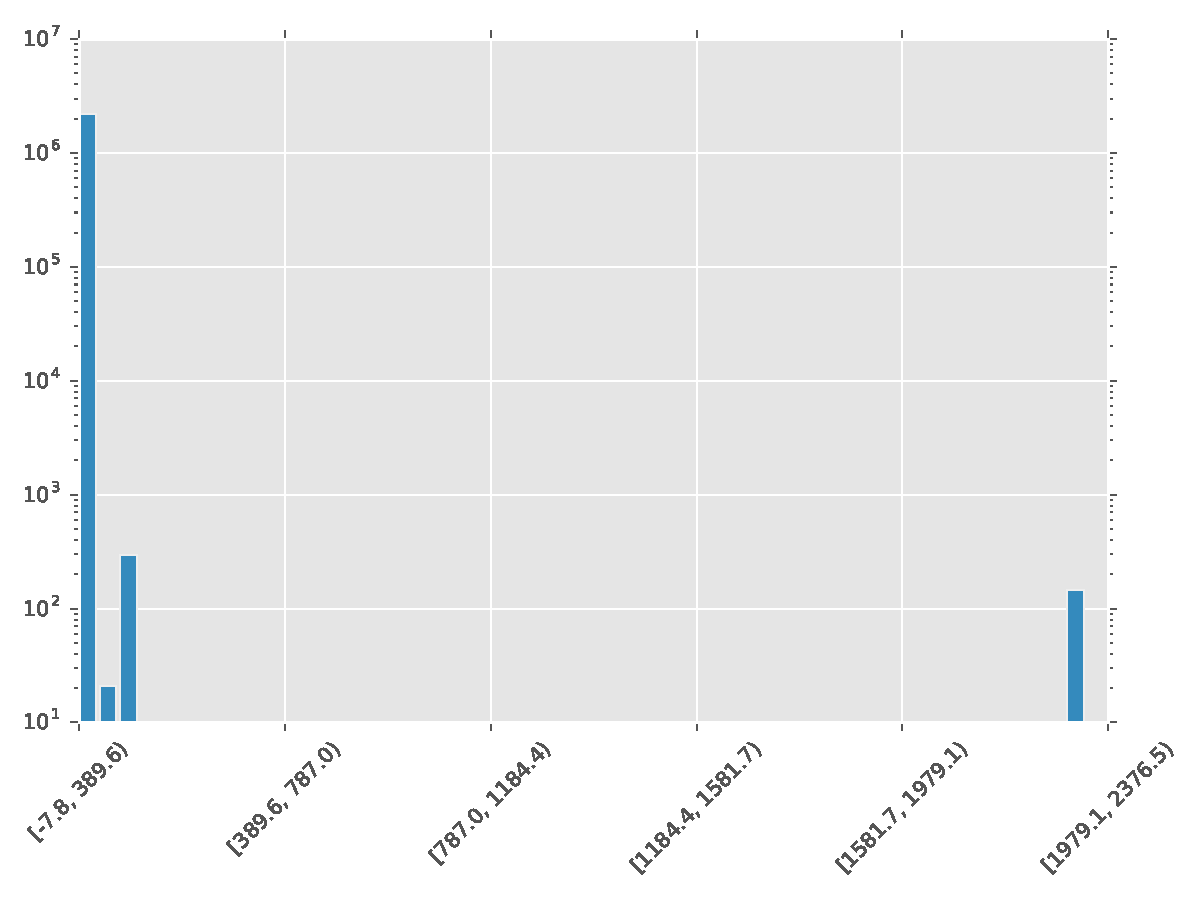
\includegraphics[width=\textwidth]{resources/histogramC}
        \caption{Histogram of weight values distribution.}
    \end{subfigure}%
    ~
    \begin{subfigure}[b]{0.32\textwidth}
        \centering
        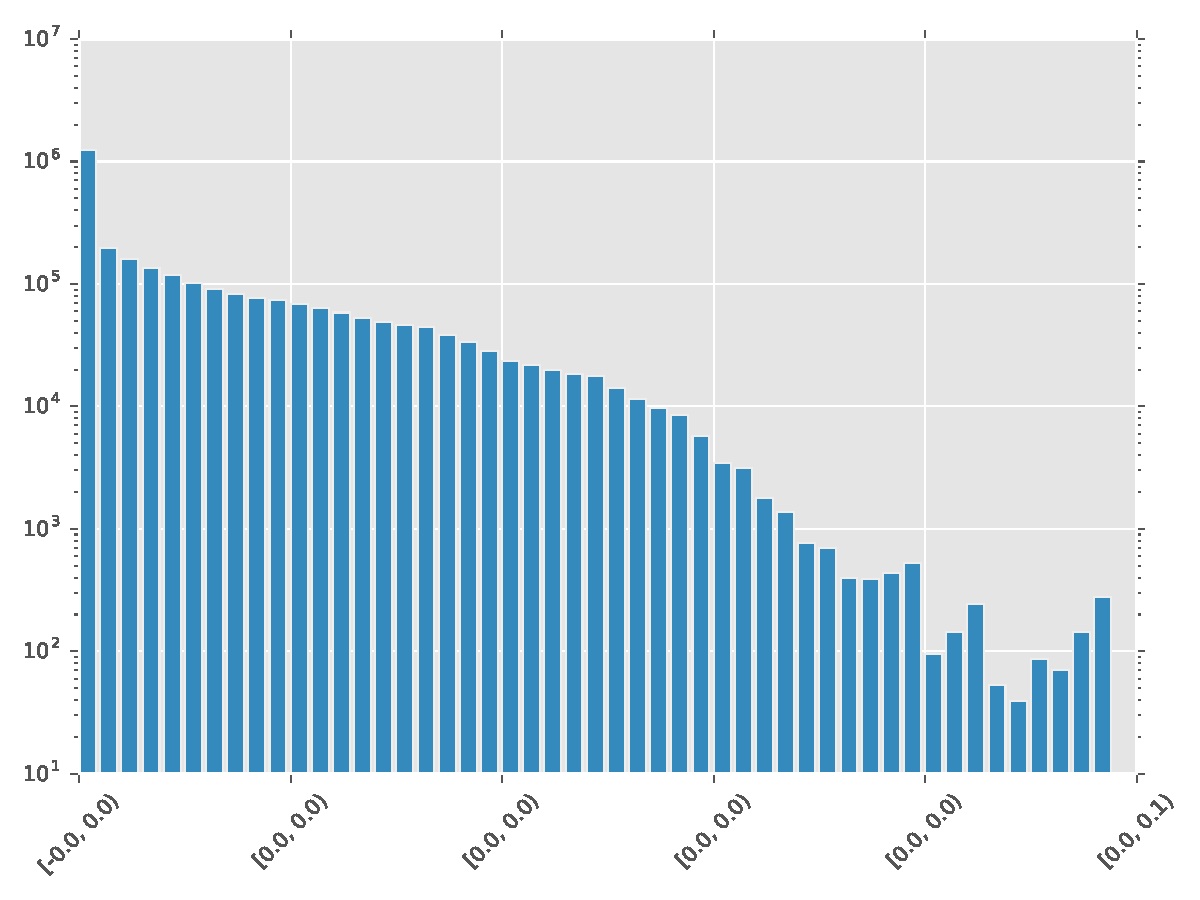
\includegraphics[width=\textwidth]{resources/histogramp}
        \caption{Histogram of pdf model values distribution.}
    \end{subfigure}
    ~
    \begin{subfigure}[b]{0.32\textwidth}
        \centering
        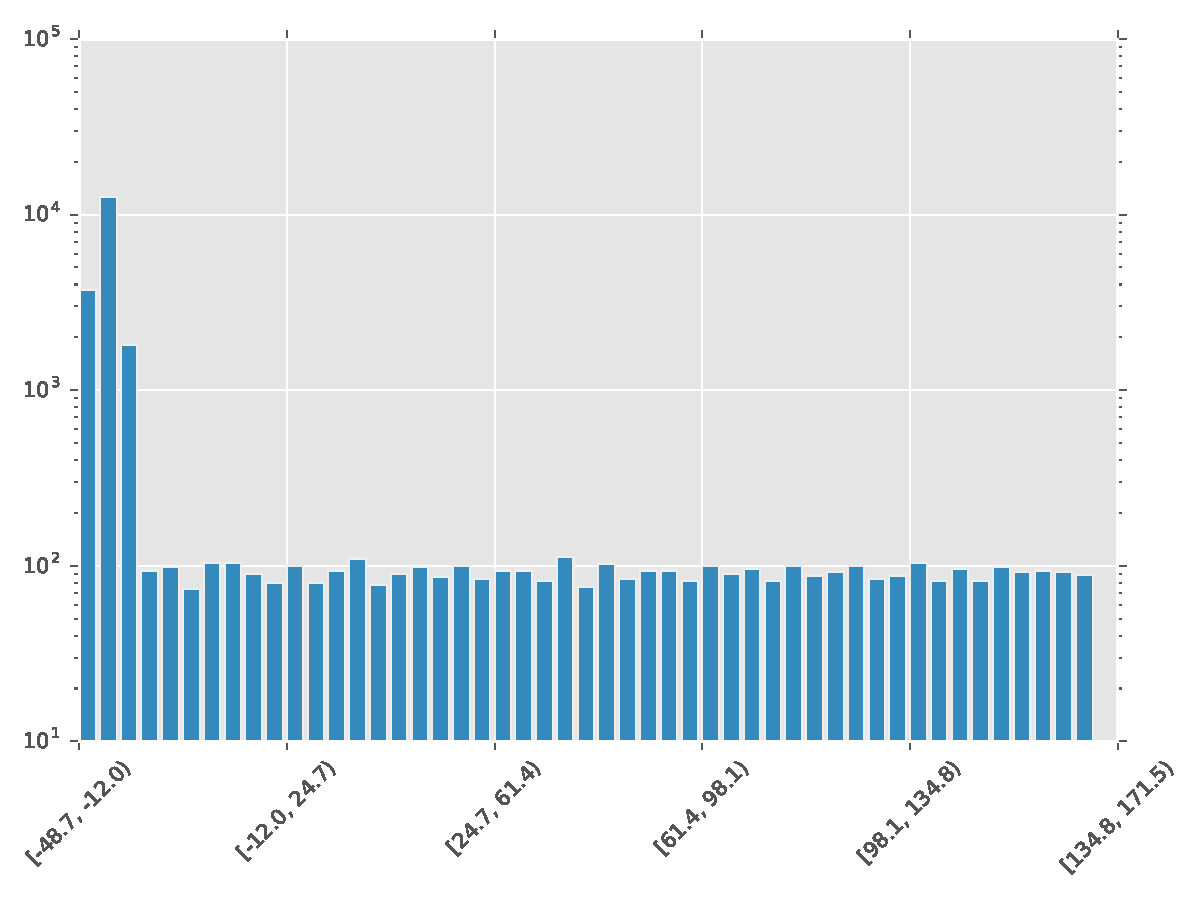
\includegraphics[width=\textwidth]{resources/histogramE}
        \caption{Histogram of E. kernel values distribution.}
    \end{subfigure}
    \caption{Value distributions}
    \label{fig:value-distributions}
\end{figure}


\begin{table}[H]
    \centering
    \caption{The final ranges}
    \label{tab:final-ranges}
    \begin{tabular}{lll}
        \toprule
        \textbf{Value set} & \textbf{Range Min} & \textbf{Range Max} \\
        \midrule
        Weight      &  \num{-2048}  &  \num{2048}     \\
        PDF model   &  \num{-1/8}   &  \num{1/8}      \\
        E. kernel      &  \num{-1/512} &  \num{1/512}    \\
        \bottomrule
    \end{tabular}
\end{table}

The speed-up that was measured with a fixed-point implementation based on the \texttt{int32\_t} type, and all values using the largest range (\num{2048}) was about \num{18} to \num{18.6} times kernel speed-up.
The problem is getting a faster conversion from the different ranges and a quick division that respects the fixed point nature of the values in the \texttt{int32\_t} datatype.
Instead of doing a normal integer division, although adding a shift to the nominator should give correct results.
To implement fixed-point math properly the project would need parts of boost for the operator overloads to create a good class, so all the errors and other debugging issues go away.
But linking boost just for that is a step too far for this project.
It was decided to drop the fixed point implementation.

After some benchmarking we found that a 4 way f32 mult takes about 9 cycles, a 4 way 32 mult takes about 5 cycles, and 8 way 16 bit mult takes 3 cycles.

\end{document}